\section{Конструкторская часть}

\subsection{Постановка задачи проектирования}

Подсистема работы с текстовыми данными на географической карте <<Вохв-Гео>> позволяет проводить накопление и анализ новостных документов с помощью формализованного языка запросов для отображения на карте. Данная подсистема предназначена для исследовательской деятельности и для включения в состав сложных комплексов анализа событий в новостных потоках.

Подсистема «Волхв-Гео» должна выполнять следующие функции
\begin{itemize}
\item Удаленный доступ к системе. Программное изделие должно обеспечивать удаленный доступ на получение информации к системе через Web-сервер.
\item Соединение с базой данных. Программное изделие должно осуществлять удаленное соединение с базой данных.
\item Ввод с клавиатуры. Данные, вводимые с клавиатуры должны иметь тип и формат, соответствующий типу и формату полей записи.
\item Добавление информации в базу данных. Программное изделие должно осуществлять добавление новой записи в базу данных при условии, что эта запись удовлетворяет всем требованиям, налагаемым на входные данные.
\item Удаление информации из базы данных. Программное изделие должно осуществлять исключение выбранной пользователем записи в таблице из исходной базы данных.
\item Редактирование информации в базе данных. Функция должна осуществлять редактирование поля записи, выбранного пользователем. При этом при редактировании данных должны выполняться все требования, налагаемые на входные данные.
\item Геотегирование новостей.
\item Анализ динамики новостей.
\item Отображение данных на карте. Функция должна осуществлять отображение новостной информации на карте.
\item Создание пользовательских сценариев. Функция должна обеспечивать создание и редактирование сценария – набора визуальных элементов на карте.
\item Создание аналитической заметки. Функция должна обеспечивать создание и редактирование аналитической заметки – текстового сопровождения к сценарию
\end{itemize}

\clearpage
\subsection{Описание предметной области}
\subsubsection{Естественно-языковая модель предметной области}

На данный момент существует очень мало систем, позволяющих проводить работу с новостными данными на географических картах. Ближайшие аналоги предоставляют отображение на карте новостной информации, предоставленной пользователями, собранной и обработанной в ручном режиме.

Подсистема <<Волхв-Гео>> должна работать в составе более крупной АИС, обеспечивая отображение собранных новостных данных на карте и должна предоставлять инструментарий по прогнозированию ситуаций и построению аналитических заметок. Подсистема использует формализованные запросы для решения задачи геотегирования текстов: формализованный запрос может определять географические привязки новостных сообщений путем учета упоминаемых географических названий. К результатам такого запроса можно привязать географические метки, чтобы использовать их в более сложных запросах.

Для реализации этой задачи требуется база новостей и система полнотекстового поиска по индексированным документам, которая не входит в структуру проектируемой подсистемы и является внешней системой, обозначаемой ИПС.

Требования, накладываемые на ИПС:
\begin{itemize}
\item Поддержка полнотекстового индекса
\item Поддержка полнотекстовых запросов
\item Поддержка запросов с учётом морфологии языка
\item Поддержка сохранённых запросов
\item Возможность редактирования документов посредством программного интерфейса
\item Поддержка текстовых меток
\end{itemize}

Подсистема Волхв-Гео, используя сохранённые в своей базе запросы, опрашивает ИПС. Полученные документы помечаются соответствующей геометкой. Используя запросы, сохранённые в ИПС, подсистема Волхв-Гео получает документы по требуемым темам и сохраняет агрегированные значения в собственной базе для последующего анализа.
По агрегированным значениям из собственной базы подсистема проводит анализ и результаты анализа сохраняются для дальнейшего использования аналитиком.

Первичной задачей является разметка документов геометками. За исключением случаев, когда координаты места события предоставлены в тексте новости, невозможно в автоматическом режиме точно привязать событие к конкретной точке земной поверхности.

Поэтому представляется нецелесообразным использование в качестве меток географических координат -- широты и долготы. В процессе проектирования было принято решение в качестве минимального географического объекта принять субъекты первого уровня, в рамках подсистемы называемые <<провинциями>>. Например, для Российской Федерации это соответствует субъекту федерации, для США -- штату, для Армении -- марзу.

Согласно стандарту ISO 3166, каждому государству соответствует двух и трёхбуквенный код, а каждому субъекту первого уровня -- код, состоящий из кода страны и кода субъекта.
Код страны/субъекта является текстовой меткой, используемой в подсистеме.

Для провинций, присутствующих в стандарте используется код из стандарта. Для провинций не присутствующих в стандарте, в основном это непризнанные территории, вводится собственное кодовое обозначение по методике, принятой в стандарте.

Результатом работы пользователя в подсистеме является сценарий развития ситуации, и аналитическая записка.

Сценарий представляет из себя набор графических элементов карты с сопроводительным текстом.

Аналитическая записка включает в себя текстовое описание текущей ситуации, сценария развития ситуации и иную информацию по необходимости.

Предметная область разработанной автоматизированной системы представлена на
рисунке~\ref{figure:domain}.

\begin{figure}[!h]
\centering
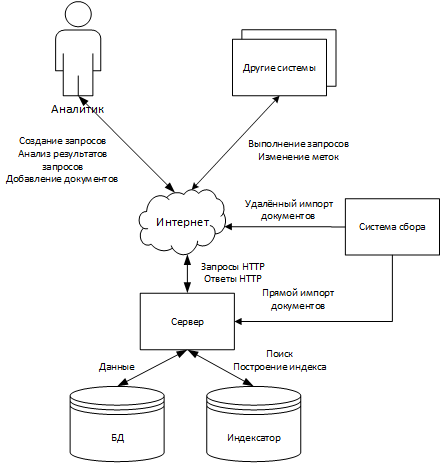
\includegraphics{design/domain}
\caption{Схема предметной области АИС.}
\label{figure:domain}
\end{figure}

\subsubsection{Сущности предметной области}

В процессе предварительного анализа предметной области были выделены следующие основные сущности:
\begin{itemize}
\item Запрос;
\item Прогноз;
\item Регион;
\item Страна;
\item Провинция;
\item Сценарий;
\item Аналитическая записка;
\end{itemize}

\subsubsection{Перечень процессов, подлежащих автоматизации}
Автоматизации подлежат следующие процессы системы:
\begin{itemize}
\item Разметка документов базы геометками;
\item Прогнозирование новостных потоков;
\item Построение сценария развития ситуации;
\item Создание аналитической записки;
\end{itemize}

\subsubsection{Выбор и обоснование критериев качества}

Для данного программного изделия можно выделить следующие критерии качества:
\begin{itemize}
\item Удобство пользовательского интерфейса;
\item Качество геотегирования;
\item Автоматическая работа;
\item Удобство интеграции с другими системами;
\item Наличие прогнозирующих функций;
\item Возможность создания пользовательских сценариев.
\end{itemize}

\paragaph{Удобство пользовательского интерфейса.}
Означает простоту и понятность работы с системой. Оценивается:
\begin{itemize}
\item структура сайта (доступ к любой странице сайта требует не более трех кликов);
\item наличие сквозного меню (меню, которое присутствует на каждой странице сайта);
\item присутствие на всех страницах сайта ссылки на главную страницу;
\item иерархическая структурированность информации сайта, степень интуитивно понятного меню;
\end{itemize}

\paragraph{Качество полнотекстового поиска.}
Оценка релевантности найденной информации, скорость выполнения запроса, возможности формализованного языка запросов.

\paragraph{Дизайн рубрикатора.}
При оценке дизайна рубрикатора документов учитывается:
\begin{itemize}
\item Непосредственное наличие рубрикатора в стандартной поставке системы;
\item Стиль отображения древовидной структуры;
\item Отображение сохранённых запросов внутри рубрик;
\item Отображение информации о количестве документов в рубрике;
\end{itemize}

\paragraph{Удобство интеграции с другими системами.} 
Оценивается:
\begin{itemize}
\item Наличие интеграционного интерфейса;
\item Удобность этого интерфейса для разработчиков;
\item Полнота интерфейса (полная реализация всех возможностей системы в интерфейсе).
\end{itemize}

\paragraph{Возможность отмечать документы метками.}
Наличие возможности отмечать произвольными метками документы или сложность реализации такой возможности. Включает в себя:
\begin{itemize}
\item Поиск по наличию меток или по их отсутствию;
\item Удобство отображения для пользователя;
\item Возможность пользователю задавать метки документам;
\item Удобство интеграционного интерфейса для работы с метками.
\end{itemize}

\paragraph{Качество прогноза.}
При оценке качества прогноза новостного потока учитывается:
\begin{itemize}
\item Построение графиков количества документов, соответствующих сохранённому запросу, по дням;
\item Наличие ретроспективного прогноза;
\item Отображение аналитической функции прогноза;
\item Качество прогнозирования, возможность прогнозировать сложные потоки;
\end{itemize}

Присвоим критериям качества следующие весовые коэффициент, которые отображены в таблице~\ref{table:qualityWeights}.

\begin{table}[h!]
\centering
\caption{Критерии качества и их весовые коэффициенты}
\label{table:qualityWeights}
\begin{tabular}{L{10cm}|C{3cm}}
\multicolumn{1}{C{10cm}|}{Критерий} & 
\multicolumn{1}{C{3cm}}{$\alpha$} \\
\hline\hline

Удобство пользовательского интерфейса & 0.1 \\
Качество полнотекстового поиска & 0.4 \\
Дизайн рубрикатора & 0.1 \\
Удобство интеграции & 0.2 \\
Возможность отмечать документы метками & 0.1 \\
Качество прогноза & 0.1 \\

\end{tabular}
\end{table}

Выполнено следующее условие:
\begin{equation}
\sum \alpha_i = 0.1 + 0.4 + 0.1 + 0.2 + 0.1 + 0.1 = 1
\end{equation}

\subsubsection{Перечень задач, подлежащих решению в процессе разработки}

В процессе разработки необходимо решить следующие задачи:
\begin{itemize}
\item исследование и анализ предметной области;
\item анализ и определение критериев качества;
\item определение функциональных требований для разрабатываемой системы;
\item разработка структуры модулей системы, с выделением функциональности для каждого модуля;
\item проектирование базы данных: инфологической и даталогической модели;
\item оптимизация структуры базы данных;
\item рассмотрение и обоснование архитектурных особенностей реализации системы;
\item выбор программных библиотек для реализации модулей;
\item разработка интерфейса взаимодействия пользователя с программой;
\item реализация графа диалога;
\item написание и отладка программного кода модулей системы;
\item разработка технической документации.
\end{itemize}

\subsubsection{Анализ аналогов и прототипов}

Для расчета нормированного значения j-го варианта по i-ому критерию необходимо
воспользоваться формулой~\ref{equation:criteria}.

\begin{equation}
\label{equation:criteria}
K_{ij} = \frac{x_{ij} - x_i^-}{x_i^+ - x_i^-}
\end{equation}
\begin{ESKDexplanation}
\item[где ] $x_{ij}$ - натуральное значение;
\item       $x_i^+$ - максимальное значение;
\item       $x_i^-$ - минимальное значение.
\end{ESKDexplanation}

Для расчета интегрального показателя необходимо воспользоваться формулой~\ref{equation:criteriaTotal}.

\begin{equation}
\label{equation:criteriaTotal}
K = \sum_{i=1}^m \alpha_i K_{ij}
\end{equation}
\begin{ESKDexplanation}
\item[где ] $m$ - количество критериев.
\end{ESKDexplanation}

Оценка по критериям производится путём присуждения баллов в соответствии со шкалой, представленной в таблице~\ref{table:criteria}.

\begin{table}[h!]
\centering
\caption{Критерии качества и их весовые коэффициенты}
\label{table:criteria}
\begin{tabular}{L{4cm}|C{2cm}|C{2cm}|C{2cm}|C{2cm}|C{2cm}}
\multicolumn{1}{C{4cm}|}{Качественный показатель} & 
\multicolumn{1}{C{2cm}|}{Отлично} & 
\multicolumn{1}{C{2cm}|}{Хорошо} & 
\multicolumn{1}{C{2cm}|}{Удовлетворительно} & 
\multicolumn{1}{C{2cm}|}{Плохо} & 
\multicolumn{1}{C{2cm} }{Неудовлетворительно} \\
\hline\hline

Количественный показатель & 5 & 4 & 3 & 2 & 1 \\
$K_{ij}$ & 1 & 0.75 & 0.5 & 0.25 & 0 \\

\end{tabular}
\end{table}

Исследуем три системы аналогов:
\begin{itemize}
\item Elsatic search
\item Mircrosoft search server
\item ODB Text
\end{itemize}

Эти аналоги имеют ряд принципиальных недостатков и не могут отвечать всем
требованиям.

Недостатками аналога «Elsatic search» являются:
\begin{itemize}
\item отсутствие системы прогнозирования;
\item отсутствие готового интерфейса пользователя.
\end{itemize}

Недостатками аналога «Mircrosoft search server» являются:
\begin{itemize}
\item малое количество возможностей у формализованного языка запросов;
\item отсутствие сохранённых запросов в рубрикаторе;
\item отсутствие системы прогнозирования.
\end{itemize}

Недостатками аналога «ODB Text» являются:
\begin{itemize}
\item невозможность интеграции системы в комплекс;
\item слабая система прогнозирования;
\item отсутствие возможности отмечать документы метками;
\end{itemize}

Сравним аналоги и прототипы без учета весовых коэффициентов, результаты сведены в таблицу~\ref{table:analogs1}.

\begin{table}[h!]
\centering
\caption{Сравнение аналогов и прототипов без учета весовых коэффициентов}
\label{table:analogs1}
\begin{tabular}{L{4cm}|C{3cm}|C{3cm}|C{3cm}|C{3cm}}
\multicolumn{1}{C{4cm}|}{Критерий} & 
\multicolumn{1}{C{3cm}|}{Elastic Search} & 
\multicolumn{1}{C{3cm}|}{Microsoft SC} & 
\multicolumn{1}{C{3cm}|}{ODB Text} & 
\multicolumn{1}{C{3cm}}{Волхв} \\
\hline\hline

Удобство пользовательского интерфейса & 1 & 4 & 5 & 4 \\ \hline
Качество полнотекстового поиска & 5 & 3 & 3 & 5 \\ \hline
Дизайн рубрикатора & 1 & 3 & 4 & 5 \\ \hline
Удобство интеграции & 5 & 3 & 1 & 4 \\ \hline
Возможность отмечать документы метками & 4 & 5 & 1 & 5 \\ \hline
Качество прогноза & 1 & 1 & 3 & 5 \\ \hline
\hline
Итого & 17 & 19 & 17 & 28 \\

\end{tabular}
\end{table}

Сравним аналоги и прототипы с учетом весовых коэффициентов, результаты сведены в таблицу~\ref{table:analogs2}.

\begin{table}[h!]
\centering
\caption{Сравнение аналогов и прототипов без учета весовых коэффициентов}
\label{table:analogs2}
\begin{tabular}{L{3cm}|C{1cm}|C{3cm}|C{2cm}|C{3cm}|C{3cm}}
\multicolumn{1}{C{3cm}|}{Критерий} & 
\multicolumn{1}{C{1cm}|}{$\alpha$} & 
\multicolumn{1}{C{3cm}|}{Elastic Search} & 
\multicolumn{1}{C{2cm}|}{Microsoft SC} & 
\multicolumn{1}{C{3cm}|}{ODB Text} & 
\multicolumn{1}{C{3cm}}{Волхв} \\
\hline\hline

Удобство пользовательского интерфейса & 0.1 & 0 & 0.75 & 1 & 0.75 \\ \hline
Качество полнотекстового поиска & 0.4 & 1 & 0.5 & 0.5 & 1 \\ \hline
Дизайн рубрикатора & 0.1 & 0 & 0.5 & 0.75 & 1 \\ \hline
Удобство интеграции & 0.2 & 1 & 0.5 & 0 & 0.75 \\ \hline
Возможность отмечать документы метками & 0.1 & 0.75 & 1 & 0 & 1 \\ \hline
Качество прогноза & 0.1 & 0 & 0 & 0.5 & 1 \\ \hline
\hline
Итого & 1 & 0.675 & 0.525 & 0.425 & 0.925 \\

\end{tabular}
\end{table}

Таким образом, автоматизированная информационная система мониторинга и
прогнозирования новостных потоков «Волхв» является лучшим среди аналогов и
оправдывает свое создание.